\chapter{QR factorisation}

\section{QR-Zerlegung}
\subsection{Definition}
Eine Matrix $A \in \mathbb{R}^{m \times n}$ , $m \ge n$ besitzt eine eindeutige QR-Zerlegung.
\begin{align}
	A = QR
\end{align}
mit einer orthogonalen Matrix $ Q \in \mathbb{R}^{m \times m} $ und einer oberen Dreiecksmatrix $ R \in \mathbb{R}^{n \times n}$ \cite{num1}

Eine QR Zerlegung kann mit einer Householder-Transformation berechnet werden.

\subsubsection{Beispiel}
Lösung eines Minimierungsproblem
\begin{align}
	\min_{x \in \mathbb{R}^n} \|Ax-b\|^2 \label{eq1}
\end{align}
mit Matrix $A \in \mathbb{R}^{m\times n}$ mit $rang(A) = n < m$ für die eine QR Zerlegung existiert.
$R$ besitzt die Gestalt 
\begin{align*}
	R=	
	\left(\begin{array}{ccc}
		*&*&* \\ 
		&*&* \\ 
		& &* \\ \hline
		& 0 &
	\end{array} \right)
	=
	\left(\begin{array}{c}
	 \\ 
	\hat{R} \\ 
	 \\ \hline
	0
	\end{array} \right) 
\end{align*}

$\hat{R}$ stellt eine obere Dreiecksmatrix dar.
Damit kann man das Minimierungs Problem wie folgt modifizieren mit $A=QR$
\begin{align}
		\min_{x \in \mathbb{R}^n} \|Ax-b\|^2 =
		\min_{x \in \mathbb{R}^n} \|Q^T(Ax-b)\|^2 =
		\min_{x \in \mathbb{R}^n} \|Rx-Q^Tb\|^2
\end{align}
Also löst
\begin{align}
Rx=Q^Tb \label{solvminqr}
\end{align}
das Minimierungsproblem (\ref{eq1}). Da $R$ eine Dreiecksmatrix ist, lässt sich (\ref{solvminqr}) leicht mit Rückwärtseinsetzen  lösen.

\section{Householder-Transformation}
Sei $v \in \mathbb{R}^n$ und $\tau \in \mathbb{R}$ dann wir die $n \times n$ Matrix 
\begin{align}
	%H = I - \tau v v^T
	H = I - 2 \dfrac{vv^T}{v^Tv}
\end{align}
als Householder-Transformation und der Vektor $v$ als Householder-Vektor bezeichnet.
Eine Householder-Transformation $H = I - 2 \dfrac{vv^T}{v^Tv}$ ist orthogonal und symmetrisch. \cite{num1}\\
Die Householder-Transformation spiegelt den Vektor $x$ auf die Achse $x_1$.
Dazu multipliziert man $H$ von links auf $x$.
\begin{align}
	Hx=\alpha e_1 \label{spiegelung}
\end{align}
mit $\alpha \in \mathbb{R}$ und $e_1$ erster kanonischer Einheitsvektor. Der Householder-Vektor steht senkrecht auf der Achse an der $x$ gespiegelt wird.\\
Die Abbildung \ref{fig:HHolder} veranschaulicht die Spiegelung der Vektors $x$ and der gestrichelt eingezeichneten Ebene auf die $x_1$ Achse.
[Abbildung \ref{fig:HHolder}]
\begin{figure}[h]
	\centering
	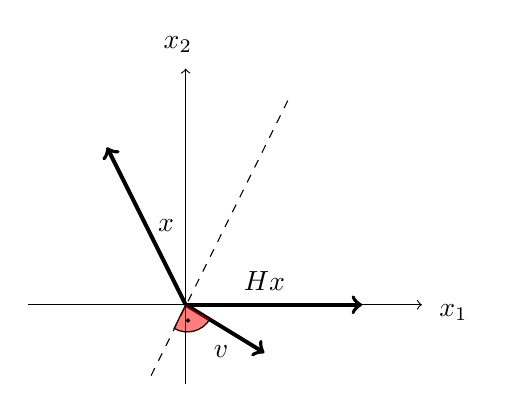
\begin{tikzpicture}

\draw[->] (-2,0) -- (3,0);
\draw[->] (0,-1) -- (0,3);

\draw[->,line width=0.5mm] (0,0) -- (-1,2);
\draw[->,line width=0.5mm] (0,0) -- (2.24,0);

\draw[dashed] (-0.44,-0.9) -- (1.34,2.68);
%\draw[->,line width=0.5mm] (0,0) -- (-0.9, 0.44);
%\draw[->,line width=0.5mm] (0,0) -- (-1,0.61);
\draw[->,line width=0.5mm] (0,0) -- (1,-0.61);





\filldraw[red, opacity=0.5] (0,0)--(-0.1467,-0.3000) arc (240:330:.3339) -- (0,0) ;
\draw[black, opacity=1] (0,0)--(-0.1467,-0.3000) arc (240:330:.3339) -- (0,0) ;
\filldraw(0.03,-0.2) circle (.02cm) ;

%Beschriftung
\draw (3.4,-0.1) node {$x_1$};
\draw (-0.1,3.3) node {$x_2$};

\draw (.45, -.6) node {$v$};
\draw (-.25, 1) node {$x$};
\draw (1,0.3) node {$Hx$};


\end{tikzpicture}
	\caption{Beispiel Householder-Transformation mit $x=(-1,2)^T$}
	\label{fig:HHolder}
\end{figure}

Eine Householder-Transformation kann die eine Matrix $A$ wie folgt transformieren.
\begin{align*}
	H_1 A= \left( 
	\begin{array}{cccc}
	* & * & * & * \\ 
	0 & * & * & * \\ 
	0 & * & * & * \\ 
	0 & * & * & *
	\end{array}
	\right)
	\quad , \quad
	H_2 H_1 A= \left( 
	\begin{array}{cccc}
	* & * & * & * \\ 
	0 & * & * & * \\ 
	0 & 0 & * & * \\ 
	0 & 0 & * & *
	\end{array}
	\right)
\end{align*} 
So erhält man folgende Faktorisierung
\begin{align*}
	R = H_{n-1} H_{n-2}\cdot ...\cdot H_1 A \Leftrightarrow A = (H_1\cdot ...\cdot H_n)R \Rightarrow Q = H_1\cdot ... \cdot H_n
\end{align*}
$Q$ ist also das Produkt aller Householder-Transformationen.


\subsection{Householder Vector}
Wie muss der Vekor $v$ aussehen damit (\ref{spiegelung}) gilt. $v \in \text{span}\{x - \alpha e_1\}$. Setze nun $v = x - \alpha e_1$ in $Hx = \alpha e_1 $ ein
\begin{align*}
	Hx =& x - \dfrac{2}{v^Tv}v(v^Tx) = x - 2\dfrac{v^Tx}{v^Tv}v\\
	=& x - \dfrac{(x - \alpha e_1)^Tx}{\|x - \alpha e_1\|^2} (x - \alpha e_1)
	=\underbrace{\left(1 - \dfrac{2(x - \alpha e_1)^Tx}{\|x - \alpha e_1\|^2}\right)}_{ \overset{!}{=} 0 } x + \alpha e_1 \dfrac{2(x - \alpha e_1)^Tx}{\|x - \alpha e_1\|^2}  \overset{!}{=} \alpha e_1
\end{align*}
Damit der Faktor vor dem $x$ verschwindet muss gelten
\begin{align*}
	1 = \dfrac{2(x - \alpha e_1)^Tx}{\|x - \alpha e_1\|^2} \Leftrightarrow (x - \alpha e_1)^T(x - \alpha e_1) = 2 x^T x - 2\alpha x_1 \Leftrightarrow \alpha = \pm \sqrt{x^Tx}
\end{align*}

Wie ist das Vorzeichen von $\alpha = \pm \sqrt{x^Tx}$ zu wählen?


\begin{algorithm}
	\caption{Housholder-Vector}
	\begin{algorithmic}
		\State $x \in \mathbb{R}^n$
	\end{algorithmic} 
	\label{alg:unblockedqr}
\end{algorithm}

\subsubsection{LAPACK QR}
Der von LAPACK benutzte Algorithmus \cite{DGEQR2}
\begin{align*}
x &= A(i+1:m,i)\\
x_1 &= A(i,i)\\
\alpha &= -1 * \text{sign}(x_1) \left|\sqrt{x_1^2 + \|x\|^2}\right|\\
\tau &= \frac{x_1 - \alpha}{\alpha} \\
v &= A(i+1:m,i) * \frac{1}{x_1 - \alpha}
\end{align*}



\subsection{Householder-Transformation anwenden}
Ein aufwändiges Matrix-Matrix Produkt kann bei der Anwendung der Housholder-Matrix $H = I - \tau vv'$ auf die Matrix A umgangen werden, indem man geschickt Klammert.
\begin{align*} 
H A =(I - \tau vv') A= A - \tau vv' A = A - \tau v*(v'*A)
\end{align*}
Statt eines Matrix-Matrix Produkts, muss man nun nur ein Matrix-Vektor Produkt und ein dyadisches Produkt berechnen.
Das Matrix-Vektor Produkt und das dyadisches Produkt haben nur einen Aufwand von $O(n^2)$.




Das führt auf den Algorithmus \ref{alg:unblockedqr}. 
\begin{algorithm}
	\caption{Ungeblockte Housholder-Transformation}
	\begin{algorithmic}
	\State $A \in \mathbb{R}^{m \times n}$
	\For {i = 0 : n}
		\State [$v$, $\tau$] = housevector($A(i:m,i)$)
		\State $w \leftarrow v^T*A$ (dgemv)
		\State $ A \leftarrow \tau * v * w + A $ (dger)
		\If {i > m}
			\State $A(i + 1 : m, j) \leftarrow v(2 : m - i + 1)$
		\EndIf
	\EndFor	
\end{algorithmic} 
\label{alg:unblockedqr}
\end{algorithm}



Der Algorithmus \ref{alg:unblockedqr} überschreibt die Matrix $A$ mit $R$. Da $R$ eine obere Dreiecksmatrix ist, werden unter der Diagonalen die Housholder-Vektoren gespeichert. A hat also die Form
\begin{align*}
	A = 
	\left(\begin{array}{ccc}
	R   &  R  & R \\ 
	v_1 &  R  & R \\ 
	v_1 & v_2 & R \\ 
	v_1 & v_2 & v_3
	\end{array} \right)
\end{align*}




%\section{Unterschiede der Algorithmen}
%Die beiden Algorithmen unterscheiden sich lediglich durch ein eine Kleinigkeite im der Transformations Matrix.
%\begin{align*}
%	H_{\text{Urban}} = I -  \dfrac{2}{v^T v}v v^T \qquad \qquad H_{\text{LAPACK}} = I - 2 \tau v v^T
%\end{align*}
%mit $\tau = \dfrac{2}{v^T v}$. Das $\tau_i$ für jeden Householder-Vektor wird in einem Vektor $\tau \in \mathbb{R}^n$ gespeichert.
%\begin{align*}
%	H_i = I - \tau_i v_i v_i^T \quad , \quad i \in 1,...,n
%\end{align*}
%
%Durch die Verwendung des $\tau$ muss das Skalarprodukts $v^T v$  nur einmalig Berechnet werde.
%
%Hypothese:\\
%Das Einsprungpotential ist nicht sehr groß.
%Das Skalar Produkt hat einen Aufwand von $O(n)$. Außerdem muss man den $v$ nicht extra in den Cache laden, da er zur Berechnung des dyadischen Produkts $vv^T$ schon im Cache liegt.



\section{QR Blocked}
Ein geblockter Algorithmus ist sinnvoll damit der Cache bei großen Matrizen optimal ausgenutzt wird. \\
%Geblockte Alorighmus
%\begin{align*}
%H &= I - VTV^T\\
%H^T &= I - VT^TV^T\\ 
%H^TA_{bs,bs} &= A_{bs,bs} - VT^TV^TA_{bs,bs}
%\end{align*}


Betrachte die Matrix $A \in \mathbb{R}^{m \times n}$ geblockt, mit einer geeigneten Blockgröße $bs$.
\begin{align}
	A = \left(\begin{array}{l|l}
	A_{0, 0} & A_{0, \text{bs}} \\ \hline
	A_{\text{bs}, 0}   & A_{\text{bs}, \text{bs}} 	
	\end{array} \right) \label{equ:blockA}
\end{align}
Die Abbildung \ref{fig:blockA} zeigt schematisch die Partitionierung von A.

Nun wird QR Zerlegung für den Block $ \left(\dfrac{A_{0, 0}}{A_{\text{bs}, 0}} \right)$
mit Algorithmus \ref{alg:unblockedqr} berechnet.
\begin{align}
	\left(\begin{array}{l} 
	A_{0, 0} \\ \hline
	A_{\text{bs}, 0}
	\end{array}\right)
	\leftarrow
	\left(\begin{array}{l} 
	Q_{0, 0}  \backslash R_{0,0} \\ \hline
	Q_{\text{bs}, 0} 
	\end{array}\right)
\end{align}

Das Bedeutet im block $A_{0, 0}$ steht nun auf und über der Diagonalen $R_{0,0}$, unterhalb der Diagonalen und im block $A_{\text{bs}, 0}$ stehen die Householder-Vektoren.

Damit 



Berechne $H_{0}$...$H_{bs}$ aus $Q_{0, 0}$ und $Q_{bs, 0}$ mit $H = I - V*T*V^T$.\\
Wende $H^T$ auf $A_{0, \text{bs}}$ und $ A_{0,\text{bs}}$ an.
\begin{align}
	\left(\begin{array}{l} 
	A_{0, \text{bs}} \\ \hline
	A_{bs, \text{bs}}
	\end{array}\right)
	\leftarrow
	H^T \left(\begin{array}{l} 
	A_{0, \text{bs}} \\ \hline
	A_{bs, \text{bs}}
	\end{array}\right)
\end{align}

Betrachte nun den Block $A_{bs, \text{bs}}$ wie in (\ref{equ:blockA}), in der Abbildung \ref{fig:blockA} gestrichelt Dargestellt.

[Abbildung \ref{fig:blockA}]
\begin{figure}
	\centering
	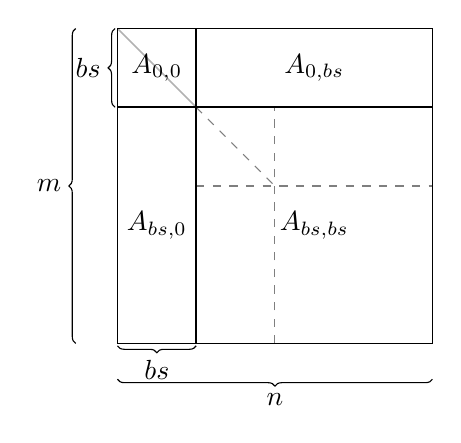
\begin{tikzpicture}
\draw[semithick] (0,0) -- (4,0) -- (4,4) -- (0,4) -- (0,0);

\draw[semithick] (1,0) -- (1,4);
\draw[semithick] (0,3) -- (4,3);
\draw[semithick,opacity=0.3] (0,4) -- (1,3);

\draw[dashed,opacity=0.5] (2,0) -- (2,3);
\draw[dashed,opacity=0.5] (1,2) -- (4,2);
\draw[dashed,opacity=0.5] (1,3) -- (2,2);


\draw (0.5,3.5) node {$A_{0,0}$};
\draw (0.5,1.5) node {$A_{bs,0}$};
\draw (2.5,3.5) node {$A_{0,bs}$};
\draw (2.5,1.5) node {$A_{bs,bs}$};
\draw[decorate, decoration={brace,mirror}, yshift=-.2ex]  (0,0) -- node[below=0.4ex] {$bs$}  (1,0);
\draw[decorate, decoration={brace}, xshift=-.2ex]  (0,3) -- node[left=0.4ex] {$bs$}  (0,4);
\draw[decorate, decoration={brace,mirror}, yshift=-3ex]  (0,0) -- node[below=0.4ex] {$n$}  (4,0);
\draw[decorate, decoration={brace}, xshift=-3.5ex]  (0,0) -- node[left=0.4ex] {$m$}  (0,4);

\end{tikzpicture}
	\caption{Partitionierung vom A}
	\label{fig:blockA}
\end{figure}

\subsection{Calc Factor T larft}

Die Funkton bekommt eine Dreiecksmatrix $V \in \mathbb{R}^{m \times k}$ einen Vektor $\tau \in \mathbb{R}^k$ und eine Matrix $T\in \mathbb{R}^{k\times k}$ übergeben. 
Die Funktion berechnet eine Dreiecksmatrix $T$ so dass
\begin{align*}
	H_1H_2...H_k = I - VTV^T \qquad \text{mit}\qquad H_i = I - \tau_i v_iv_i^T
\end{align*}

Warum und wie das Funktoniert wird hier beschreiben \cite{Joffrain:2006:AHT:1141885.1141886}.

Versuch einer Herleitung

Vorwärts \\
n=2;
\begin{align*}
	H_1 H_2 x &= (I-\tau_1 v_1 v_1^T)(I-\tau_2 v_2 v_2^T)x\\
	= &(I - \tau_1 v_1 v_1^T - \tau_2 v_2 v_2^T -  \tau_1 v_1 v_1^T \tau_2 v_2 v_2^T )x\\
  = &x - \tau_1 v_1 v_1^T x - \tau_2 v_2 v_2^T x - \tau_1 \tau_2 v_1 (v_1^T v_2 )v_2^T x\\
  = &x - \tau_1 v_1 v_1^T x - \tau_2 v_2 v_2^T x - \tau_1 \tau_2 (v_1^T v_2 ) v_1 v_2^T x\\
\end{align*}
n=3;
\begin{align*}
	H_1 H_2 H_3 x &= (I-\tau_1 v_1 v_1^T)(I-\tau_2 v_2 v_2^T)(I-\tau_3 v_3 v_3^T)x\\
	= &(I - \tau_1 v_1 v_1^T - \tau_2 v_2 v_2^T - \tau_3 v_3 v_3^T\\
    &- \tau_1 v_1 v_1^T \tau_2 v_2 v_2^T - \tau_1 v_1 v_1^T \tau_2 v_2 v_2^T \tau_3 v_3 v_3^T )x \\
  = &x - \tau_1 v_1 v_1^T x - \tau_2 v_2 v_2^T x - \tau_3 v_3 v_3^T x\\
    &- \tau_1 \tau_2 v_1 (v_1^T v_2 )v_2^T x- \tau_1 \tau_2 \tau_3 v_1 ( v_1^T v_2)( v_2^T v_3) v_3^T x \\
  = &x - \tau_1 v_1 v_1^T x - \tau_2 v_2 v_2^T x - \tau_3 v_3 v_3^T x \\
    &- \tau_1 \tau_2 (v_1^T v_2 ) v_1 v_2^T x- \tau_1 \tau_2 \tau_3 ( v_1^T v_2)( v_2^T v_3) v_1 v_3^T x \\
\end{align*}
Rückwärts\\
n=2
\begin{align*}
  H_{1,2} x &= (I - V T V^T) x = x - V T V^T x\\
  &= x - (v_1, v_2)
  \begin{pmatrix}
    a & b \\ 0 & c
  \end{pmatrix}
  \begin{pmatrix}
    v_1^T \\ v_2^T 
  \end{pmatrix}
  x\\
  &= x - (v_1, v_2)
  \begin{pmatrix}
    a & b \\ 0 & c
  \end{pmatrix}
  \begin{pmatrix}
    v_1^T x \\ v_2^T x
  \end{pmatrix}\\
  &= x - (v_1, v_2)
  \begin{pmatrix}
    a v_1^T x + b v_2^T x\\  c v_2^T x
  \end{pmatrix}\\
  &= x - v_1(a v_1^T x + b v_2^T x) - v_2 (c v_2^T x)\\
  &= x - a v_1 v_1^T x - b v_1 v_2^T x - c v_2 v_2^T x
\end{align*}
n=3
\begin{align*}
  H_{1,2,3} x &= (I - V T V^T) x = x - V T V^T x\\
  &= x - (v_1, v_2, v_3)
  \begin{pmatrix}
    a & b & c\\ 
    0 & d & e\\
    0 & 0 & f
  \end{pmatrix}
  \begin{pmatrix}
    v_1^T \\ v_2^T \\ v_3^T
  \end{pmatrix}
  x\\
  &= x - (v_1, v_2, v_3)
  \begin{pmatrix}
    a & b & c\\ 
    0 & d & e\\
    0 & 0 & f
  \end{pmatrix}
  \begin{pmatrix}
    v_1^T x \\ v_2^T x \\ v_3^T
  \end{pmatrix}\\
  &= x - (v_1, v_2, v_3)
  \begin{pmatrix}
    a v_1^t x + b v_2^t x + c v_3^t\\ 
    d v_2^T x + e v_3^T \\
    f v_3^T
  \end{pmatrix}\\
  =& x - v_1(a v_1^T x + b v_2^T x + c v_3^T x) \\ 
   & - v_2 ( d v_2^T x + e v_3^T x) \\ 
   & - v_3 ( f v_3^T ) \\
  =& x - a v_1 v_1^T x - b v_1 v_2^T x - c v_1 v_3^T x \\
   & - d v_2 v_2^T x - e v_2 v_3^T \\
   & - f v_3 v_3^T
\end{align*}
Koeffizienten Vergleich

\begin{align*}
  a &= \tau_1 \\
	b &= \tau_1 \tau_2 (v_1^T v_2) \\
	c &= \tau_2 \\
  T &=
  \begin{pmatrix}
    \tau_1 & \tau_1 \tau_2 (v_1^T v_2)\\ 0 & \tau_2
  \end{pmatrix}
\end{align*}

Produkt orthogonaler Matrizen ist orthogonal 
\begin{align*}
	A^{-1} = A^T, B^{-1} = B^T\\
	(AB)^{-1} = B^{-1}A^{-1} = B^TA^T = (AB)^T
\end{align*}
$\Rightarrow H=I-VTV^T$ ist orthogonal\\
ich bin doof Q ist ja auch orthogonal

\subsection{Apply H larfb}

Die Funktion larfb bekommt eine Dreiecksmatrix $V \in \mathbb{R}^{m \times k}$, eine Dreiecksmatrix $T \in \mathbb{R}^{k \times k}$ und eine Matrix $C \in \mathbb{R}^{m \times n }$ übergeben.
Die Funktion wendet eine  Block Reflector Matrix $ 	H = C - V T V^T $ von rechts auf die Matrix $ C $ an. 
Mit einem weiteren Übergabeparameter kann angeben werden ob die Block Reflector Matrix noch transponiert werden soll.
Die Funktion berechnet also
\begin{align*}
	C \leftarrow H C = C - V T V^T C \quad \text{oder} \quad 	C \leftarrow H^T C = C - V T^T V^T C
\end{align*}
Die Abbildung \ref{fig:patrA} zeigt die Partitionierung der Matrix A für die Funktion larfb.\\
Falls $m > k $ werden die Matrizen $V$ und $C$ aufgeteilt in $V=\left(\dfrac{V_1}{V_2}\right)$ und $C=\left(\dfrac{C_1}{C_2}\right)$. Dabei wird $V$ genau so gewählt, dass $V_1 \in \mathbb{R}^{k\times k}$ der Dreiecksteil der Matrix und quadratisch ist und $V_2 \in \mathbb{R}^{m-k\times k}$ der Rest der Matrix. Die Matrix $C$ wird in $C_1 \in \mathbb{R}^{k \times n}$ und $C_2 \in \mathbb{R}^{m-k \times n}$  aufgeteilt.\\
Die Aufteilung ist Notwendig da die BLAS-Funktion trmm (matrix-matrix product where one input matrix is triangular) nur für Quadratische Dreiecksmatrizen implementiert ist.

Im Fall $ m = k $ ist die Aufteilung nicht Notwendig da $ V $ quadratisch ist.

\begin{align*}
	(C_1^T * V_1 * T *V_1^T)^T\\
	V_1 * T^T * V_1^T * C_1
\end{align*}



Dies führt zu dem[ Algorithmus \ref{alg:applyblockref} ]\\
\begin{algorithm}
	\caption{Block reflector anwenden}
	\label{alg:applyblockref}
	\begin{algorithmic}
		\State 	$W \leftarrow C_1^T$ (copy)
		\State	$W \leftarrow W * V_1 $ (trmm)
		\If {m > k}
			\State $W \leftarrow W + C_2^T*V_2$ (gemm)
		\EndIf
		\State 	$ W \leftarrow W * T^T \quad \text{or}\quad  W * T$ (trmm)
		\If {m > k}
			\State $C_2 \leftarrow C_2 - V_2 * W^T$ (gemm)
		\EndIf
		\State 	$ W \leftarrow W * V_1^T $ (trmm)
		\State 	$ C_1 \leftarrow C_1 - W^T $
	\end{algorithmic}
\end{algorithm}


[Abbildung \ref{fig:patrA}]
\begin{figure} 
	\centering
	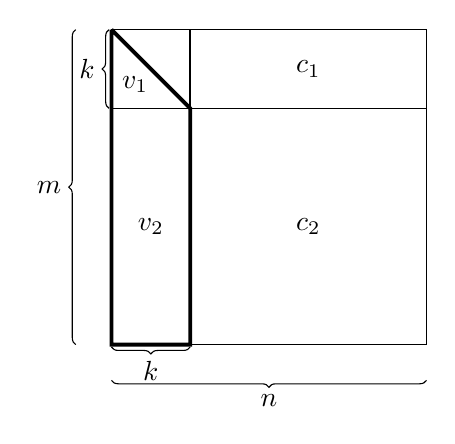
\begin{tikzpicture}
\draw[semithick] (0,0) -- (4,0) -- (4,4)-- (0,4)-- (0,0);


\draw[semithick] (1,0) -- (1,4);
\draw[semithick] (0,3) -- (4,3);
\draw[line width=0.5mm] (0,4) -- (0,0) -- (1,0) -- (1,3) -- (0,4);


\draw[decorate, decoration={brace,mirror}, yshift=-.2ex]  (0,0) -- node[below=0.4ex] {$k$}  (1,0);
\draw[decorate, decoration={brace}, xshift=-.2ex]  (0,3) -- node[left=0.4ex] {$k$}  (0,4);
\draw[decorate, decoration={brace,mirror}, yshift=-3ex]  (0,0) -- node[below=0.4ex] {$n$}  (4,0);
\draw[decorate, decoration={brace}, xshift=-3ex]  (0,0) -- node[left=0.4ex] {$m$}  (0,4);

\draw (0.3,3.3) node {$v_1$};
\draw (0.5,1.5) node {$v_2$};
\draw (2.5,3.5) node {$c_1$};
\draw (2.5,1.5) node {$c_2$};



\end{tikzpicture}
	\caption{Partitionierung vom A für larfb}
	\label{fig:patrA}
\end{figure}


\subsection{Iterativer Algorithmus}
[Algorithmus \ref{alg::italg}]
\begin{algorithm}
	\caption{Iterativer Algorithmus}
	\label{alg::italg}
	\begin{algorithmic}
		\For {i = 0 : n}
			\State QR = A;
			\If {i + ib > n}
				\State Calc T: H=I-VTV'
				\State Apply H: A=H'A
			\EndIf
		\EndFor
	\end{algorithmic}
\end{algorithm}


\subsection{Rekursiver Algorithmus}


e
